\section{Schiebeoperationen}
Erfordert use IEEE.NUMERIC\_STD.ALL;

\subsection{Logische Schiebeoperatoren SLL, SRL}

	\begin{multicols}{2}
		\begin{itemize}
			\setlength{\itemsep}{1pt}
			\setlength{\parskip}{0pt}
			\setlength{\parsep}{0pt}
			
			\item Bits werden um eine Stelle geschoben.
			\item Freiwerdende Stelle wird mit Initalwert des Basistyps aufgef�llt:
			=0.
			\item Aus dem Indexbereich hinausgeschobener Inhalt geht verloren.
		\end{itemize}
		\begin{center}
			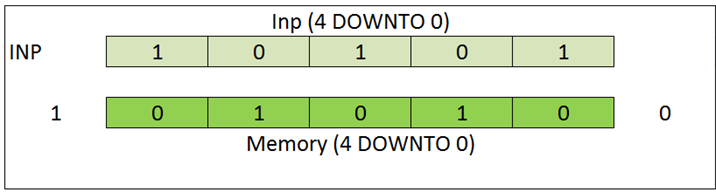
\includegraphics[width=.4\textwidth]{pics/logic_shift}
		\end{center}
	\end{multicols}
	
	\begin{multicols}{2}	
		\begin{lstlisting}[language=vhdl,tabsize=2]
			signal MEM: bit_vector (4 DOWNTO 0);
			MEM <= MEM sll 1;
		\end{lstlisting}
		
		\textbf{Anwendung:} Muliplikation / Divison mit $2^n$
	\end{multicols}
	
\subsection{Arithmetische Schiebeoperatoren SLA, SRA}
	\begin{multicols}{2}
		\begin{itemize}
			\setlength{\itemsep}{1pt}
			\setlength{\parskip}{0pt}
			\setlength{\parsep}{0pt}
			
			\item Bits werden um eine Stelle geschoben.
			\item Freiwerdende Stelle wird mit letztem geschobenem Bit aufgef�llt.
			\item Aus dem Indexbereich hinausgeschobener Inhalt geht verloren.
		\end{itemize}
		\begin{center}
			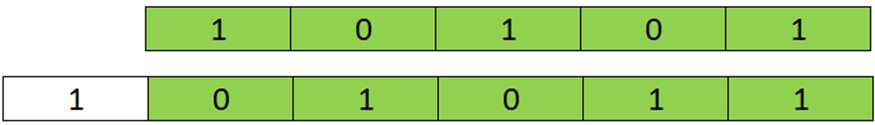
\includegraphics[width=.4\textwidth]{pics/arith_shift}
		\end{center}
	\end{multicols}
	
	\begin{multicols}{2}	
		\begin{lstlisting}[language=vhdl,tabsize=2]
			IMP <= sla 1;
		\end{lstlisting}
		
		\textbf{Anwendung:} Division mit $2^n$ bei sign-magnitude Darstellung (SRA).
	\end{multicols}

\subsection{Rotierende Schiebeoperatoren ROR, ROL}
	\begin{multicols}{2}
		\begin{itemize}
			\setlength{\itemsep}{1pt}
			\setlength{\parskip}{0pt}
			\setlength{\parsep}{0pt}
			
			\item Bits werden um eine Stelle geschoben.
			\item Freiwerdende Stelle wird mit vorderstem Bit der Kette aufgef�llt.
			\item Aus dem Indexbereich hinausgeschobener Inhalt wird hinten angeh�ngt.
		\end{itemize}
		\begin{center}
			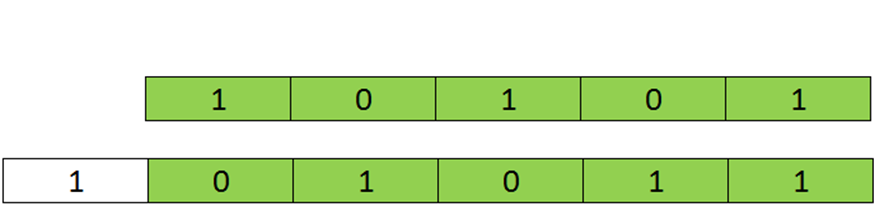
\includegraphics[width=.4\textwidth]{pics/rol_shift}
		\end{center}
	\end{multicols}
	
	\begin{multicols}{2}	
		\begin{lstlisting}[language=vhdl,tabsize=2]
			IMP <= rol 1;
		\end{lstlisting}
		
		\textbf{Anwendung:} Bitweise Analyse.
	\end{multicols}
		